%% This is file `elsarticle-template-1a-num.tex',
%%
%% Copyright 2009 Elsevier Ltd
%%
%% This file is part of the 'Elsarticle Bundle'.
%% ---------------------------------------------
%%
%% It may be distributed under the conditions of the LaTeX Project Public
%% License, either version 1.2 of this license or (at your option) any
%% later version.  The latest version of this license is in
%%    http://www.latex-project.org/lppl.txt
%% and version 1.2 or later is part of all distributions of LaTeX
%% version 1999/12/01 or later.
%%
%% The list of all files belonging to the 'Elsarticle Bundle' is
%% given in the file `manifest.txt'.
%%
%% Template article for Elsevier's document class `elsarticle'
%% with numbered style bibliographic references
%%
%% $Id: elsarticle-template-1a-num.tex 151 2009-10-08 05:18:25Z rishi $
%% $URL: http://lenova.river-valley.com/svn/elsbst/trunk/elsarticle-template-1a-num.tex $
%%
\documentclass[preprint,12pt]{elsarticle}

%% Use the option review to obtain double line spacing
%% \documentclass[preprint,review,12pt]{elsarticle}

%% Use the options 1p,twocolumn; 3p; 3p,twocolumn; 5p; or 5p,twocolumn
%% for a journal layout:
%% \documentclass[final,1p,times]{elsarticle}
%% \documentclass[final,1p,times,twocolumn]{elsarticle}
%% \documentclass[final,3p,times]{elsarticle}
%% \documentclass[final,3p,times,twocolumn]{elsarticle}
%% \documentclass[final,5p,times]{elsarticle}
%% \documentclass[final,5p,times,twocolumn]{elsarticle}

%% if you use PostScript figures in your article
%% use the graphics package for simple commands
%% \usepackage{graphics}
%% or use the graphicx package for more complicated commands
%% \usepackage{graphicx}
%% or use the epsfig package if you prefer to use the old commands
%% \usepackage{epsfig}

%% The amssymb package provides various useful mathematical symbols
\usepackage{amssymb}
%% The amsthm package provides extended theorem environments
%% \usepackage{amsthm}

%% The lineno packages adds line numbers. Start line numbering with
%% \begin{linenumbers}, end it with \end{linenumbers}. Or switch it on
%% for the whole article with \linenumbers after \end{frontmatter}.
%% \usepackage{lineno}

%% natbib.sty is loaded by default. However, natbib options can be
%% provided with \biboptions{...} command. Following options are
%% valid:

%%   round  -  round parentheses are used (default)
%%   square -  square brackets are used   [option]
%%   curly  -  curly braces are used      {option}
%%   angle  -  angle brackets are used    <option>
%%   semicolon  -  multiple citations separated by semi-colon
%%   colon  - same as semicolon, an earlier confusion
%%   comma  -  separated by comma
%%   numbers-  selects numerical citations
%%   super  -  numerical citations as superscripts
%%   sort   -  sorts multiple citations according to order in ref. list
%%   sort&compress   -  like sort, but also compresses numerical citations
%%   compress - compresses without sorting
%%
%% \biboptions{comma,round}

% \biboptions{}


%\journal{Nuclear Physics B}

%\begin{document}

%\begin{frontmatter}

%% Title, authors and addresses
\usepackage{graphics}
%\usepackage{amsmath}
\usepackage[dvips]{color}
\usepackage{epsfig}
\usepackage{float}
\usepackage{latexsym,amsfonts,amsmath,amssymb,graphicx}
\usepackage{eucal, amssymb,amsmath,graphicx, amsfonts, latexsym}
\usepackage[left=3cm,right=3cm,top=1.5cm,bottom=1.5cm]{geometry}
% Over-full v-boxes are due to the \v{c} in author's name
\vfuzz2pt % Don't report small over-full v-boxes

% THEOREM Environments ------------------------------------
\newtheorem{thm}{Theorem}[subsection]
\newtheorem{cor}[thm]{Corollary}
\newtheorem{lem}[thm]{Lemma}
\newtheorem{prop}[thm]{Proposition}
%\theoremstyle{definition}
\newtheorem{defn}[thm]{Definition}
%\theoremstyle{remark}
\newtheorem{rem}[thm]{Remark}
\numberwithin{equation}{subsection}
% MATH ----------------------------------------------------
\DeclareMathOperator{\RE}{Re}
\DeclareMathOperator{\IM}{Im}
\DeclareMathOperator{\ess}{ess}
\newcommand{\eps}{\varepsilon}
\newcommand{\To}{\longrightarrow}
\newcommand{\h}{\mathcal{H}}
\newcommand{\s}{\mathcal{S}}
\newcommand{\A}{\mathcal{A}}
\newcommand{\J}{\mathcal{J}}
\newcommand{\M}{\mathcal{M}}
\newcommand{\W}{\mathcal{W}}
\newcommand{\X}{\mathcal{X}}
\newcommand{\BOP}{\mathbf{B}}
\newcommand{\BH}{\mathbf{B}(\mathcal{H})}
\newcommand{\KH}{\mathcal{K}(\mathcal{H})}
\newcommand{\Real}{\mathbb{R}}
\newcommand{\Complex}{\mathbb{C}}
\newcommand{\Field}{\mathbb{F}}
\newcommand{\RPlus}{\Real^{+}}
\newcommand{\Polar}{\mathcal{P}_{\s}}
\newcommand{\Poly}{\mathcal{P}(E)}
\newcommand{\EssD}{\mathcal{D}}
\newcommand{\Lom}{\mathcal{L}}
\newcommand{\States}{\mathcal{T}}
\newcommand{\abs}[1]{\left\vert#1\right\vert}
\newcommand{\set}[1]{\left\{#1\right\}}
\newcommand{\seq}[1]{\left<#1\right>}
\newcommand{\norm}[1]{\left\Vert#1\right\Vert}
\newcommand{\essnorm}[1]{\norm{#1}_{\ess}}
% -----------------------------------------------------------
\begin{document}

\title{Gene flow model in a forest for Dogwood}


\author{ D. M. Chan, E.L. Foster, and R. J. Dyer }

\address{Department of Mathematics and Applied Mathematics,
1015 Floyd Ave., Richmond, VA 23284}

%\email{dmchan@vcu.edu}

\thanks{This work was completed with the support of NSF.}

%\subjclass{Primary 47A15; Secondary 46A32, 47D20}

%\keywords{linear operator, invariant subspace, transitive algebra}

\date{\today}



% -----------------------------------------------------------

\begin{abstract}
The understanding of gene movement in plant species is critical to the
management of both plant and animal species reliant on that plant.
Pollen is the mechanism by which plants pass their genetic material from one
generation to the next. Pollen dispersal studies have focused
primarily on purely random diffusion processes, while this may be a good
assumption for species pollinated mainly by abiotic means, such as
wind, it is most likely an over simplification for species that are pollinated
by biotic means, such as insects \cite{Chan}.

Correlated random walk (CRW) models are a model of animal movement
\cite{Prasad05} and have been successfully used to explore the movement of
animals in varying ecological contexts \cite{Bartumeus07}. An agent-based model
(ABM) is developed to describe pollen movement via insects as
a correlated random walk (CRW). This model is used to explore how insect path
lengths and pollen distribution are affected by the varying
turning angle and plant density.

\end{abstract}

% -----------------------------------------------------------
\maketitle
% -----------------------------------------------------------

\section{{\bf Introduction}}
Pollen is the mechanism by which plants pass their genetic material from one
plant to the another. Two modes of transporting pollen, from one plant to
another, include abiotic (wind dispersal) and biotic (animal dispersal).
Understanding the methods by which pollen spreads across the landscape is
important for management of both plant and animal species. Understanding the
pollination process may allow for optimization of the number of pollinators used
for crop pollination, thereby reducing cost to farmers. Additionally, a better
understanding of the pollination process can lead to the prevention of cross
pollination of genetically modified plant species and non-genetically modified
plant species.

Pollen dispersal studies, for both abiotic and biotic pollen dispersal, have
focused primarily on purely random diffusion processes, while this may be a good
assumption for species pollinated by wind, it is most likely an over
simplification for species that are pollinated by animals \cite{Chan}. A purely
random diffusion process in two dimensions accurately predicts pollen dispersal
at a particular time, but only for a purely random walk \cite{Byers01}.

Pollen movement via biotic means may not be a purely random process and
therefore would not diffuse in a purely random fashion. In fact, there are
several examples of pollinating animals that exhibit \emph{trap line} behavior
\cite{Chan}. That is, they follow a particular route as they collect pollen.
Thus the movement of animals as they carry pollen may follow more direct paths
and therefore would not result in a purely random diffusion process
\cite{Cresswell03}. Such behaviors result in dispersal that does not mimic a
purely random walk. The movement of animals can be described as a correlated
random walk (CRW), where the correlation is based on the distribution and
magnitude of random turning angles. In this way the previous direction of travel
influences the direction of travel for the next step.

A purely random walk can be used to model a purely random diffusion process such
as Brownian motion \cite{Codling}. While a CRW can be used as a general model of
animal movement \cite{Prasad05} and have been successfully used to explore the
movement of animals in varying ecological contexts \cite{Bartumeus07}. CRW
models have been used to model the dispersal of bark beetles, Coleoptera:
Scolytidae \cite{Byers01}, deterministic diffusion \cite{Klages}, and fractional
Brownian motion \cite{Enriquez}.

An agent-based model (ABM) describing pollen movement via animals as a
correlated random walk (CRW) is introduced. ABMs consist of agents that interact
with each other and their environment. ABMs allow for simulations that consist
of a large number of interacting parts that would not be easily constructed
otherwise \cite{Fioretti05}. Agents can represent things such as people, animals,
organizations, etc. that interact with each other and their environment. The
environment in an ABM can represent things such as a spatial domain, or a
network in which the agents are connected to each other \cite{Gilbert}. ABMs
have been used in modeling racial segregation, supply chain dynamics, and neural
networks \cite{Gilbert}.

Consequences of the CRW and the interaction of animals with plants is examined
using computer simulations. Two animals statistics (\emph{average path distance}
and \emph{average maximum distance}) and three plant statistics (\emph{average
pollination distance}, \emph{average maximum pollination distance}, and
\emph{average weighted diversity of fathers}) are presented. Turning angle and
plant density are varied and their effects on animals paths and pollen
distribution are examined.

It is shown that bias can be introduced by describing animal movement as a
purely random walk. That is, there is a significant difference between the model
outcomes for a purely random walk as compared to a CRW. Thus, modeling animal
mediated pollen dispersal by way of a purely random diffusion process is likely
to result in errors in the approximation of the extent of pollen dispersal.


\section{{\bf Methods}}
An agent-based correlated random walk model was built using the java based ABM
package REPAST\cite{REPAST}. The model assumes continuous space and consists of
two interacting agents; \emph{animals} and \emph{plants}. The plants are
considered point sources (i.e. radius of a plant is zero) that release pollen to
the animals. Animals transport the pollen across the environment, and at each
step, $j$, animals move from one location to the next. As the animal moves about
the environment it searches for plants to collect and deposit pollen. The number
of plants is determined by $n = \lfloor\omega \cdot A\rfloor$, where $\omega$ is
the density of plants, and $A$ is the area of the environment.

\subsection{\emph{Movement}}
The movement of animals in this model can be described by three stages: (1)
\emph{searching} stage - an animal is moving about the environment in search of
plants within a radius of $r$; (2) \emph{movement to plant} stage - an animal
has located a plant and moves to the plant; (3) \emph{movement from plant}
stage- an animal has visited a plant and moves away from the plant. Movement
transitions from the \emph{searching} stage to \emph{movement to a plant} stage
to the \emph{movement away from a plant} stage and then back to the
\emph{searching} stage and so on. Each one of these stages have particular
animal behaviors associated with them.

Animals in this study are considered to be solitary and do not display social
behavior, thus no central hives or nesting areas are considered. Each animal
starts at random locations throughout the environment. Initially the $i^{th}$
animal selects a direction of travel, $\theta^{\left(i\right)}_0$, between
$0^{\circ} \mbox{ and } 360^{\circ}$ sampled from a uniform distribution. Here
$0^\circ$ is in the direction of increasing $x_1$ values. Once an initial
direction of travel is selected the animal begins to move in the selected
direction. Animals move in incremental steps; the length and direction are
updated at the beginning of each step. Let the location of the $i^{th}$ animal
for the $j^{th}$ step be given by the coordinate pair
$\mathbf{X}^{\left(i\right)}_j=\left(x^{\left(i\right)}_{1,j},
x^{\left(i\right)}_{2,j}\right)$, where $\mathbf{X}^{\left(i\right)}_0$ is the
$i^{th}$ animals starting location. The $i^{th}$ animal's location at step
$j=1,2\dots$ is determined based on its location at step $j-1$, step size
($s^{\left(i\right)}_j$), the previous direction of travel
($\theta^{\left(i\right)}_{j - 1}$), and the random turning angle
($\delta^{\left(i\right)}_j$). The direction of travel is updated at each step
by adding a new heading to the previous direction of travel and is determined by
the formula
\[
	\theta^{\left(i\right)}_j = \theta^{\left(i\right)}_{j-1} +
\delta^{\left(i\right)}_j
\]
Thus, during any stage the $j^{th}$ location of an animal is given recursively
by
\[
	\mathbf{X}^{\left(i\right)}_j = \mathbf{X}^{\left(i\right)}_{j-1} +
s^{\left(i\right)}_j \cdot
		\left(\cos \theta^{\left(i\right)}_j, \sin
\theta^{\left(i\right)}_j \right)
\]

\begin{figure}[H]\label{TurningAngle}
	\begin{center}
	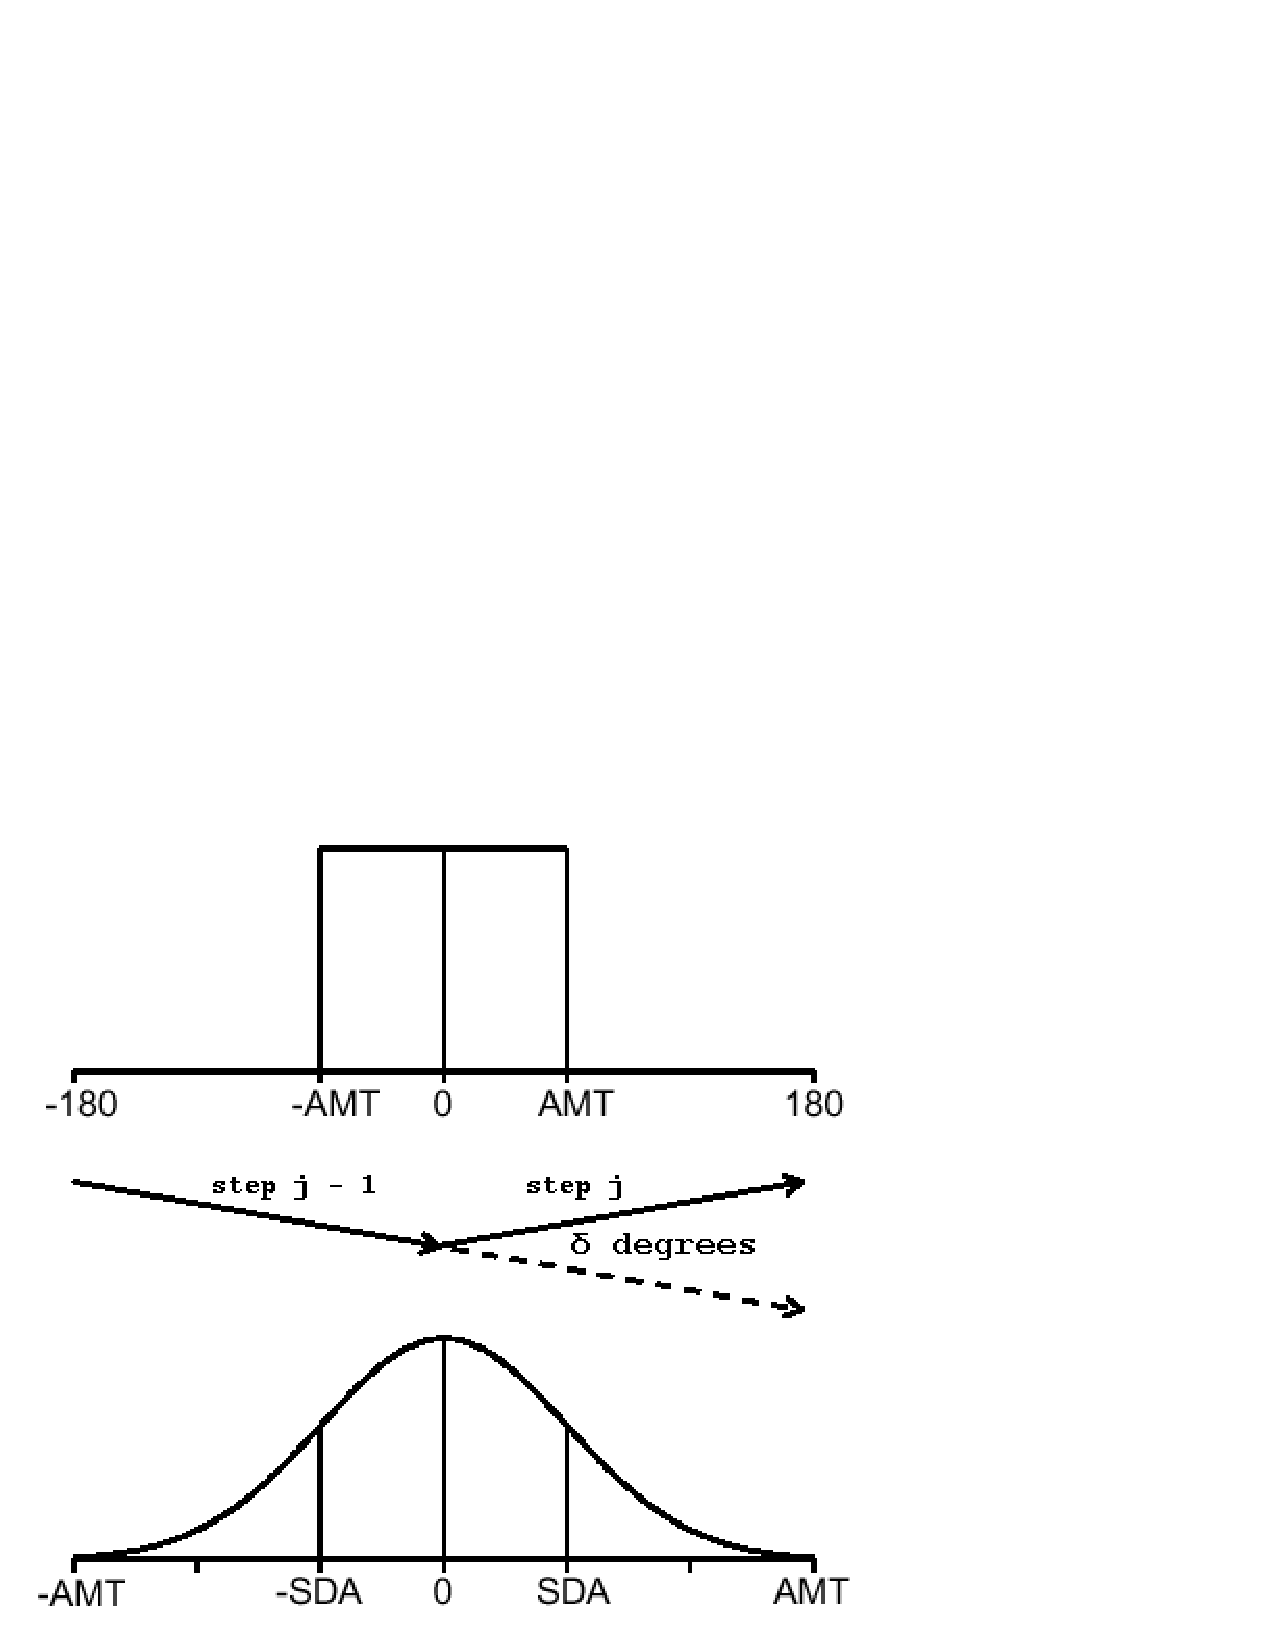
\includegraphics[width=1.0\textwidth]{TADistribution.pdf}
	\end{center}
	\caption{Turning Angle for (a) uniform distribution and (b) depiction
	of what a path may look like.}
\end{figure}

As in \cite{Byers01}, a uniform distribution of angles within a left or right
angle of maximum turn (AMT) is used for turning angles,
$\delta^{\left(i\right)}_j$. The turning angle is sampled from a uniform
distribution in the interval $\left[-AMT, AMT\right]$, where $0^\circ \le AMT
\le 180^\circ$.The direction of travel is updated differently for each
particular movement stage. Animals in the \emph{movement to a plant} stage move
in the direction of the selected plant, while an animal is in the \emph{movement away
from a plant} stage the direction of travel is selected uniformly from the
interval $\left[0^{\circ}, 360^{\circ}\right]$.

During the \emph{searching} stage, animals take steps of size
$s^{\left(i\right)}_j$ between each location and ``looks'' for nearby plants.
During the \emph{movement to a plant} stage the step size is equal to the
distance from the animal's current location to the plant's location, and during
the \emph{movement from a plant} stage $s^{\left(i\right)}_j$ is some number
greater than the search radius $r$. The animal must move a distance greater than
the search radius to ensure it doesn't continually move back to the same plant.
The distance between each step can either be fixed or variable, the length of
which is determined by which stage of movement the animal is in. For a fixed
step size; $s^{\left(i\right)}_j = 1$ for the \emph{searching} stage, and
$s^{\left(i\right)}_j = r + 0.01$ during the \emph{movement from a plant} stage.
If the step size is variable, $s^{\left(i\right)}_j$ is sampled uniformly from
the interval $[0, 1]$ for the \emph{searching} stage, and $(r, r + 1]$ during
the \emph{movement from a plant} stage.

\subsection{\emph{Pollination}}
When an animal is on a plant, it collects pollen, distributes pollen, and
consumes food. Each plant contains a number of flowers, $\phi$, from which an
animal may obtain pollen. When an animal visits a plant it picks up pollen from
one or more flowers. The number of flowers from which an animal can obtain
pollen is determined by the total number of flowers on a plant, the fraction of
flowers in bloom at any one time ($a$), the number of times ($j$) the plant has
previously been visited by an animal, and the maximum fraction of flowers
available for pollination ($\eta$). The formula for the number of total flowers
available for visitation during a $k^{th}$ visit to the $j^{th}$ plant
($f_{j,k}$) is given by
\begin{equation}\label{flowers}
	f_{j,k} = \phi \cdot a \cdot \eta^k.
\end{equation}
Let $f_j$ be the total number of flowers visited at the $j^{th}$ plant, then if
one adds up the number of flowers, given by (\ref{flowers}), over $m$ visits one
obtains the series
\[
	f_j = \sum_{k=1}^{m} f_{j,k} = \phi \cdot \sum_{k=1}^{m} a \cdot
\eta^{k}.
\]
Now letting $\hat{f}_j$ be the theoretical limit of flowers to be visited at the
$j^{th}$ plant. Then $\hat{f}_j$ is given by the convergent geometric series
\begin{equation} \label{limit}
	\hat{f}_j = \lim_{m \to \infty} \sum_{k=1}^{m} f_{j,k} = \phi \cdot
\frac{a \cdot \eta}{1 - \eta}
\end{equation}
for $0<\eta<1$.

It is assumed that the amount of food eaten and the amount of pollen collected
is proportional to the number of visited flowers. An animal collects pollen and
eats from every flower that it visits, and so the amount of pollen collected and
the amount of food eaten is proportional to the equation (\ref{flowers}). Let
$f^{\left(i\right)}_{j,k}$ be the number of flowers visited by the $i^{th}$
animal during the $k^{th}$ visit to the $j^{th}$ plant then the amount of
polllen/nectar in the $i^{th}$ animal's stomach after $m$ plant visits is given
by
\[
	c^{\left(i\right)}_m = \sum_{j=0}^{m} \beta f^{\left(i\right)}_{j,k},
\]
where $\beta$ is the proportionallity constant for the amount of pollen
collected at a plant. %The total amount of food that an animal can eat is limited
%by the stomach size, $c_{max}$.

In the field it is observed that a fraction of all flowers are pollinated
($\alpha$), then there is an associated probability that a flower is pollenated
($\rho$), where
\begin{equation} \label{Prob}
	\alpha = \rho \cdot \hat{f}_k.
\end{equation}
Using equation (\ref{limit}) and (\ref{Prob}) we can determine the probability
that a flower is pollinated, $\rho$, by the formula
\[
	\rho = \frac{\alpha}{\phi} \cdot \frac{1 - \eta}{a \cdot \eta}.
\]

If it has been determined that a flower should be pollinated we must determine
which previous plant should pollinate that flower. Each flower visited is
recorded and is available to pollinate the current flower, except those flowers
that are on the same plant. Self- pollination, is not considered, because the
likelyhood of self-pollination is low due to mechanisms that impeded
self-pollination. Each flower considered has an equal likelihood of pollinating
the current flower. Once the animal has visited a plant and
collected/distributed pollen it then moves away from the plant, thereby
transitioning briefly back into the \emph{movement from a plant} stage, where
the animal selects a new random direction between $0^\circ$ and $360^\circ$ from
a uniform distribution. Then the animal transitions back into the
\emph{searching} stage, and so on.

\subsection{Time and Stopping Criteria}
Let the velocity an animal travels ($v$) be fixed, and the time spent at a plant
($t_{plant}$) be fixed then the travel time for an animal will be given by the
formula
\[
	t^{\left(i\right)} = \frac{s^{\left(i\right)}}{v} + T^{\left(i\right)}
\cdot t_{plant},
\]
where $T^{\left(i\right)}$ is the number of plants visited by the $i^{th}$
animal. If we let the maximum allowable travel time be $t_{max}$ then once
$t^{\left(i\right)} \geq t_{max}$ or $c^{\left(i\right)}_m \geq c_{max}$ the
animal is removed from the simulation. When there are no animals left the
simulation terminates.

\subsection{\emph{Model Statistics}}
The consequences of the correlated random walk and the interaction of animals
with plants is examined using computer simulations. In this study the following
statistics are calculated; \emph{Average Path Distance}, \emph{Average Maximum
Distance} which are animal properties, and \emph{Average Pollination Distance},
\emph{Average Maximum Pollination Distance}, \emph{Average Weighted Diversity of
Fathers} which are plant properties. These statistics can give a better insight
into how genes flow between plants.

\subsubsection*{\emph{Average Path Distance}}
The total distance the $i^{th}$ animal travels, which will be called the path
distance, $s^{\left(i\right)}$, is determined by adding each step distance
together. Therefore, the path distance for the $i^{th}$ animal, after $n$ steps,
is given by
\begin{equation} \label{pathD}
	s^{\left(i\right)} = \sum_{j=1}^n s^{\left(i\right)}_j.
\end{equation}
The \emph{average path distance} is a measure of the total travel distance
covered during a pollination trip averaged over all animals. The \emph{average
path distance} is affected by both the plant density and turning angle. This is
because the stopping criteria includes time spent at plants and so if an animal
encounters more plants it would be expected to reach the maximum time stopping
criteria %or the maximum stomach criteria
and travels a shorter distance. One
determines the \emph{average path distance} by averaging path distances over all
animals
\[
	\bar{s} = \frac{1}{b} \sum_{i=1}^b s^{\left(i\right)},
\]
where $s^{\left(i\right)}$ is the path distance for the $i^{th}$ animal and $b$
is the total number of animals in the simulation.

\subsubsection*{\emph{Average Maximum Distance}}
The maximum distance for an animal is the largest distance from the animal's
initial starting location, $\left(x_{1,0}, x_{2,0}\right)$, to a point traveled
to by the animal. Therefore, the $i^{th}$ animal's maximum distance is given by
\[
		M^{\left(i\right)} = \max_j \sqrt{\left(x^{\left(i\right)}_{1,0}
- x^{\left(i\right)}_{1,j}\right)^2 +
			\left(x^{\left(i\right)}_{2,0} -
x^{\left(i\right)}_{2,j}\right)^2},
\]
where $\left(x^{\left(i\right)}_{1,j}, x^{\left(i\right)}_{2,j}\right)$ is the
$i^{th}$ animal's $j^{th}$ location. This is then averaged over all animals
using the formula
\[
	\bar{M} = \frac{1}{b} \sum_{i=1}^b M^{\left(i\right)}.
\]

\subsubsection*{\emph{Average Pollination Distance}}
The \emph{average pollination distance} is the average distance pollen travels
from father to mother. If the location of the $i^{th}$ plant be given by the
ordered pair $\left(x^{\left(i\right)}_1, x^{\left(i\right)}_2\right)$ then the
pollination distance for the $i^{th}$ plant to the $j^{th}$ plant is given by
\[
	p^{\left(i\right)}_j = \sqrt{\left(x^{\left(i\right)}_1 -
x^{\left(j\right)}_1\right)^2 + \left(x^{\left(i\right)}_2 -
		x^{\left(j\right)}_2\right)^2}.
\]
The \emph{average pollination distance} for each plant is then averaged over all
plants using the formula
\[
	\bar{p} = \frac{1}{n} \sum_{i=1}^{n} \left(
\frac{1}{\tau^{\left(i\right)}} \sum_{j=1}^{\tau^{\left(i\right)}}
p^{\left(i\right)}_j
		\right),
\]
where $\tau^{\left(i\right)}$ is the total number of seeds for the $i^{th}$
plant. This tells us the average distance pollen travels from father to mother.

\subsubsection*{\emph{Average Maximum Pollination Distance}}
The \emph{average maximum pollination distance} is the average of the largest
distances a pollen grain has traveled to each mother plant. The maximum distance
from mother to father is first calculated for $i^{th}$ mother using the formula
\[
	P^{\left(i\right)} = \max_j p^{\left(i\right)}_j.
\]
Once the maximum pollination distance for each plant has been calculated for
each mother we then average this over all mothers using the formula
\[
	\bar{P} = \frac{1}{n} \sum_{i=1}^{n} P^{\left(i\right)}.
\]

\subsubsection*{\emph{Average Weighted Diversity of Fathers}}
The Weighted Diversity of Fathers is a measure of the number of distinct fathers
that contribute pollen to a mother and is given by the formula
\[
	\hat{F}^{\left(i\right)} =
\frac{1}{\left(\tau^{\left(i\right)}\right)^2}
\sum_{j=1}^{\Delta\tau^{\left(i\right)}} F^2_{j,i},
\]
where $\Delta\tau^{\left(i\right)}$ is the number of different fathers
contributing pollen to the $i^{th}$ plant, and $F_{j,i}$ is the number of times
the $j^{th}$ father has contributed pollen to the $i^{th}$ plant. The weighted
diversity of fathers is then averaged over all mothers
\[
	E = \frac{1}{n} \sum_{i=1}^n 1/\hat{F}^{\left(i\right)}.
\]

\subsection{\emph{Turning Angle and Plant Density Effects on Animal and Plant
Statistics}}\label{EffectOnStats}
Finally, we examine the effects of turning angles and plant densities on our
various model statistics. %While the analysis of the previous simulations focused
%on animal density distributions, the simulations described here will evaluate the
Here the simulations described will evaluate the effects of both turning angle and plant density have on pollination. In the
simulation presented 1,000 animals are randomly distributed through out our
environment and allowed to move for 1,200 seconds at a speed of 1 unit of
distance per second and variable step size. The time spent at each plant was set
to 100 seconds and so a theoretical maximum of 12 plants could be visited,%. The
%maximum stomach size was set to 75,
while $a = 0.2, r = 0.7 \mbox{ and } \rho =
0.3$ based on the field report from \cite{Gathman} \cite{Raine}. The simulations
were run 10 times and all statistics were averaged over the 10 runs.

% -----------------------------------------------------------
\section{{\bf Results}}
The results are presented in two parts: first, the effects of movement
parameters and plant density on animal density distributions; second, the
effects of movement parameters and plant density on our model statistics
(\emph{Average Path Distance}, \emph{Average Maximum Distance}, and
\emph{Average Pollination Distance}, \emph{Average Maximum Pollination
Distance}, \emph{Average Weighted Diversity of Fathers}).

\subsection{\emph{Examination Effects of Turning Angle and Plant Density on
Model Statistics}}
The evaluation that follows focuses primarily on the affects of both turning
angle and plant density have on pollination. The following model parameters were
held constant; $a = 0.2$, $\eta = 0.75 $, $\phi = 100$, $\rho = 0.4286$, $v =
1.0$, $n = 1000$, $r = 1.0$, $A = 101 \times 101$, $t_{max} = 1200$, and
$t_{plant} = 100$. While 10 simulations were run for each pair of $AMT$ and
$\omega$. Where $AMT$ was varied over $[0^\circ, 15^\circ, 30^\circ, 45^\circ,
60^\circ, 90^\circ, 135^\circ, 180^\circ]$ and $\omega$ was varied over $[0.01,
0.03, 0.05, 0.07, 0.10, 0.15]$. The data presented will not have standard error
(SE) in the plots due to the small size of each SE. The SEs were all less than
1\% of average. The SE was calculated by dividing the sample standard deviation
(SD) by the square root of the total number of samples. This was used instead of
SD, since the error was applied to the average.

{\emph{Average Path Distance}}
\begin{figure}
  \begin{center}
  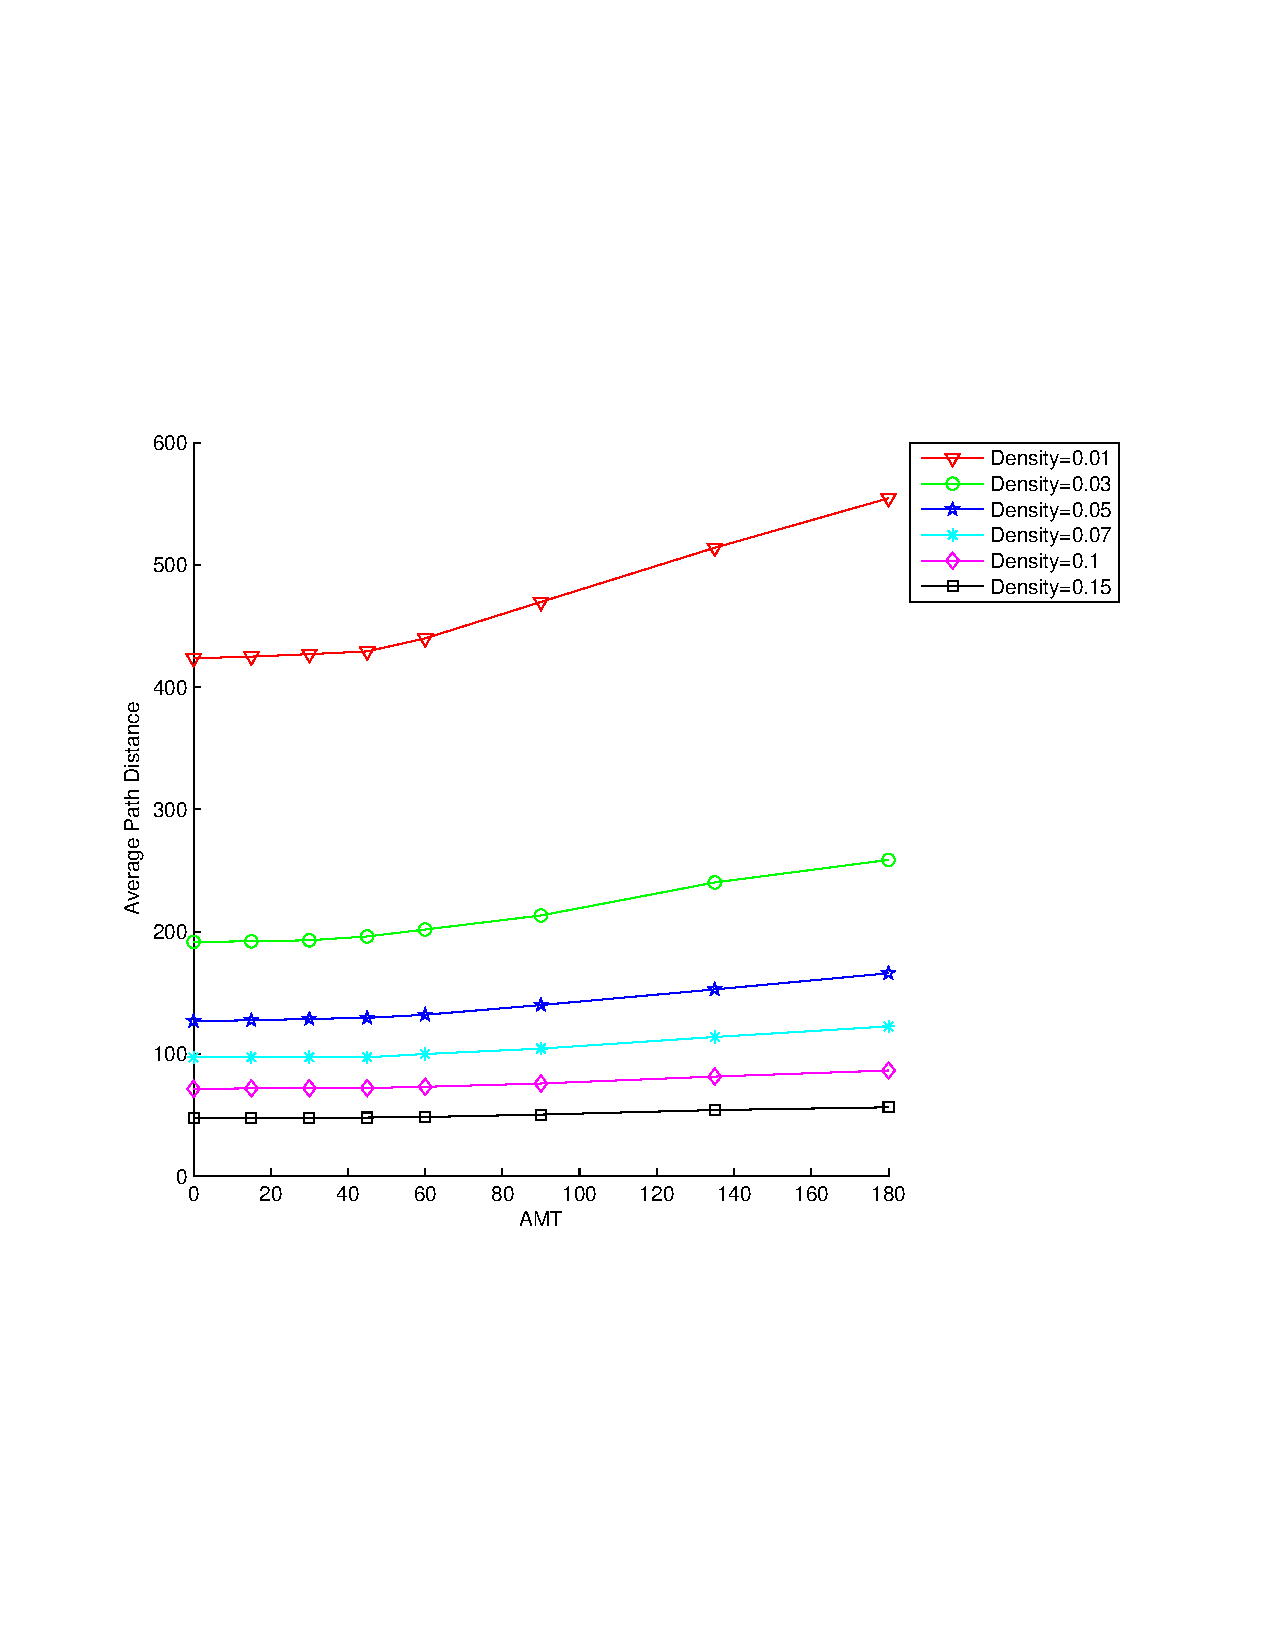
\includegraphics[width=1.0\textwidth]{PathVsAMT.pdf}
  \end{center}
  \caption{\small Average Path Distance vs. Turning Angle for Various Plant
Densities}
  \label{AvgPathN}
\end{figure}

In {\bf Figure} \ref{AvgPathN} the plant density has a much greater affect on
the average path distance over that of the turning angle. The effects from
turning angle only seem to be significant for the lowest of densities. This is
likely due to more plants being visited in a shorter path distance, and
therefore animals meet the stopping criteria in shorter path distances.

It should also be noted that under the model assumptions with enough animals it
is possible for the plants to essentially run out of pollen. This is more likely
for high animal population and low plant densities. %If this occurs the animals
%will continue searching for food until the maximum time stopping criteria is
%reached, whereas for high plant densities the stopping criteria reached would be
%due to the stomach criteria.

\subsubsection*{\emph{Average Maximum Distance}}
\begin{figure}
  \begin{center}
  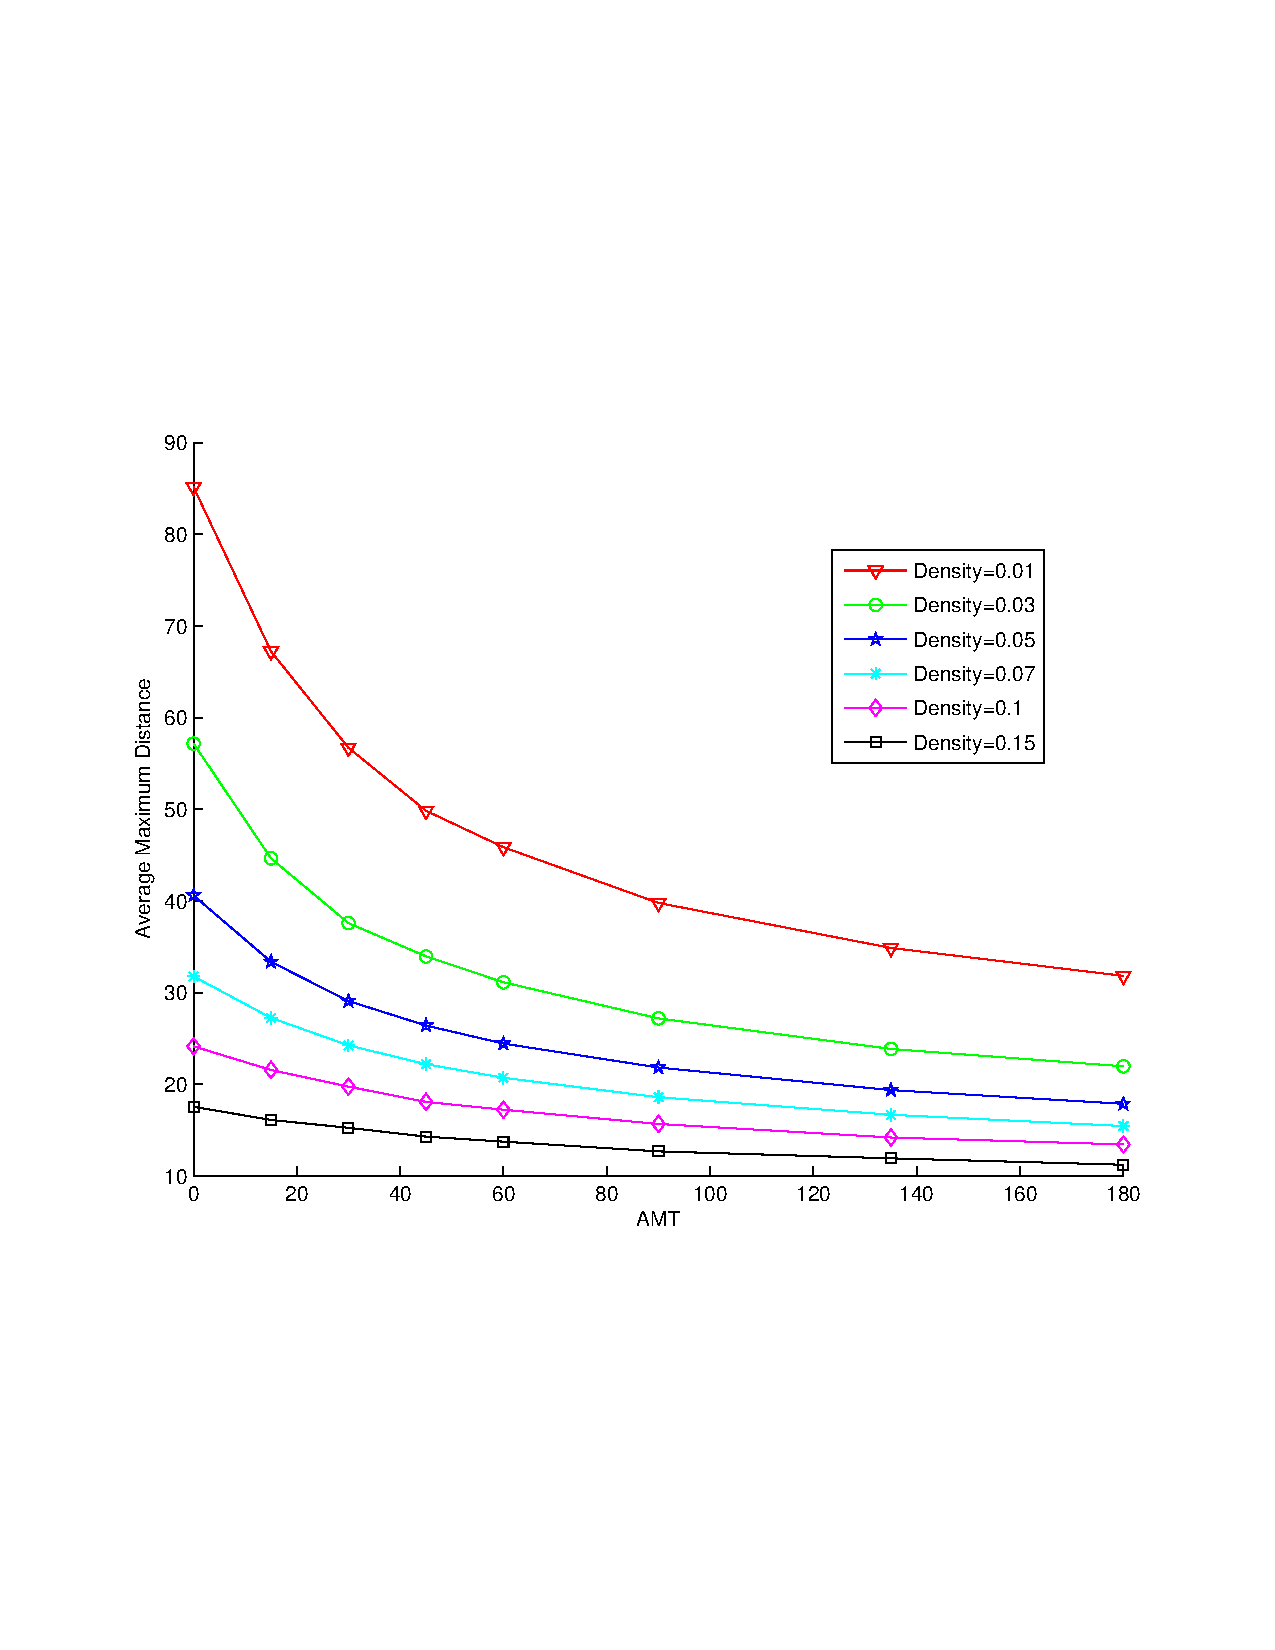
\includegraphics[width=1.0\textwidth]{MaxDVsAMT.pdf}
  \end{center}
  \caption{\small Average Maximum Distance vs. Turning Angle for Various Plant
Densities}
  \label{AvgMaxDBees}
\end{figure}

From {\bf Figure} \ref{AvgMaxDBees} the average maximum distance an animal
travels is clearly affected by both the turning angle and plant density. As the
plant density decreases the average maximum distance increases as one might
expect, since animals travel farther distances between plants. Also, as the
turning angle decreases the average maximum distance increases. This too is what
one might expect, since as the turning angle decreases the animals are traveling
along a straighter path and therefore will travel farther before turning. For a
plant density of 0.01 and AMT = $0^\circ$ the average maximum distance is
quadruple of the average maximum distance for a plant density of 0.01 and AMT =
$180^\circ$. For a higher plant density of 0.15 the average maximum distance is
50\% larger. Thus, a purely random diffusion process results in shorter average
maximum distances as compared to smaller turning angles, and as was seen with
the average pollination distance the effect of turning angle is more pronounced
for smaller plant densities. Again, this is expected since for higher plant
densities the animal direction is reset more often and therefore the animal path
becomes more and more like a purely random walk.

\subsubsection*{\emph{Average Pollination Distance}}
\begin{figure}
  \begin{center}
  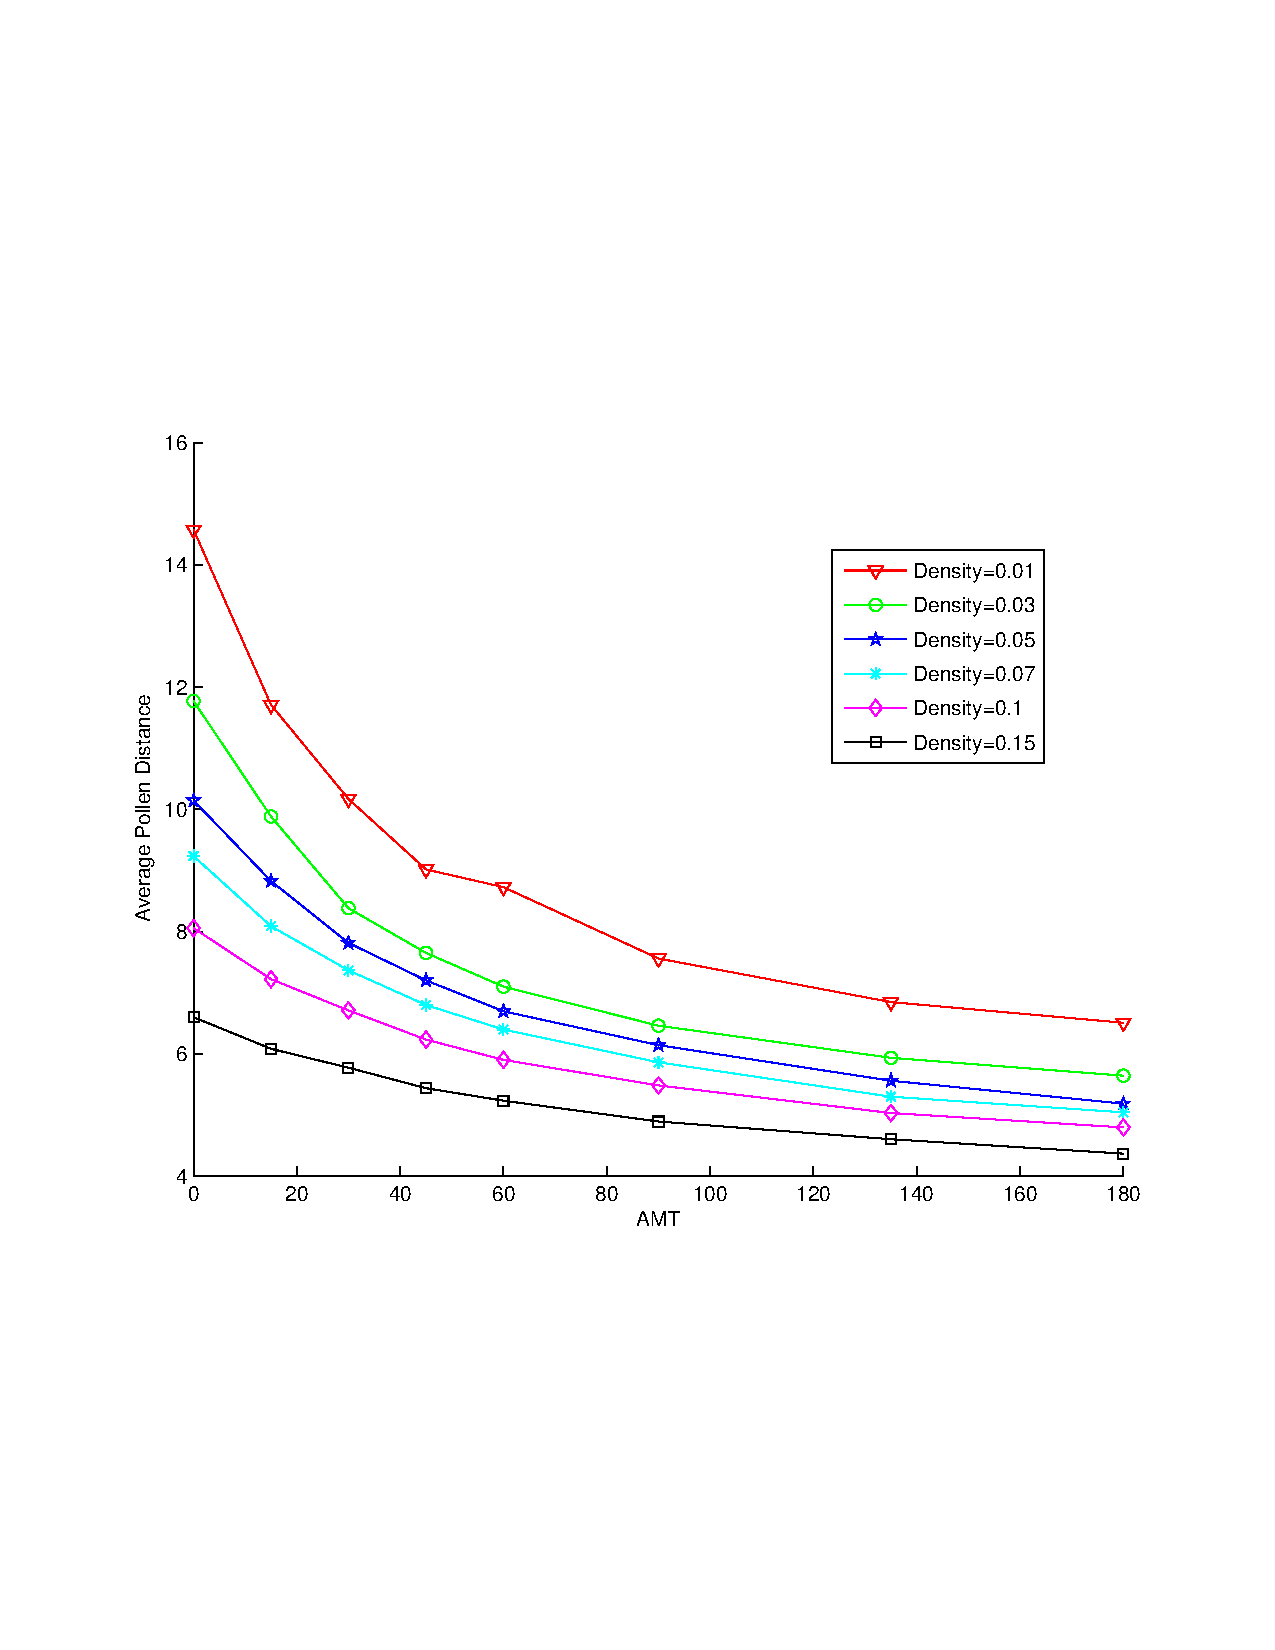
\includegraphics[width=1.0\textwidth]{PollenDVsAMT.pdf}
  \end{center}
  \caption{\small Average Pollination Distance vs. Turning Angle for Various
Plant Densities}
  \label{AvgDist}
\end{figure}
The average pollination distance is clearly affected by both the turning angle
and the plant density as one can see from {\bf Figure} \ref{AvgDist}. For a
plant density of 0.01 and AMT = $0^\circ$ the average maximum pollination
distance is approximately triple of that for the same plant desnity and AMT =
$0^\circ$. Additionally, for plant density of 0.15 and AMT = $0^\circ$ the
average pollination distance is approximately double of the average pollination
distance for the same density and AMT = $180^\circ$. Therefore, the average
pollination distance for wind dispersal is less than that of an average
pollination distance for an animal that follows a straighter path despite the
plant densities simulated.

Density does have an affect on the average pollination distance. For an AMT =
$45^\circ$ the average pollination distance for a plant density of 0.01 is
approximately double of the average pollination distance for an the same turning
angle and a plant density of 0.15. This is due to plants being closer together
for higher densities, and therefore an animal travels a shorter distance to
visit the same number of plants. Thus, the average pollination distance clearly
decreases as density increases. If the the pollination distance decreases it is
expected that the ability of a plant to spread its genes across a large spatial
area is reduced. Thus, a plant is only able to mate with other plants in a
shorter distance.

\subsubsection*{\emph{Average Maximum Pollination Distance}}
\begin{figure}
  \begin{center}
  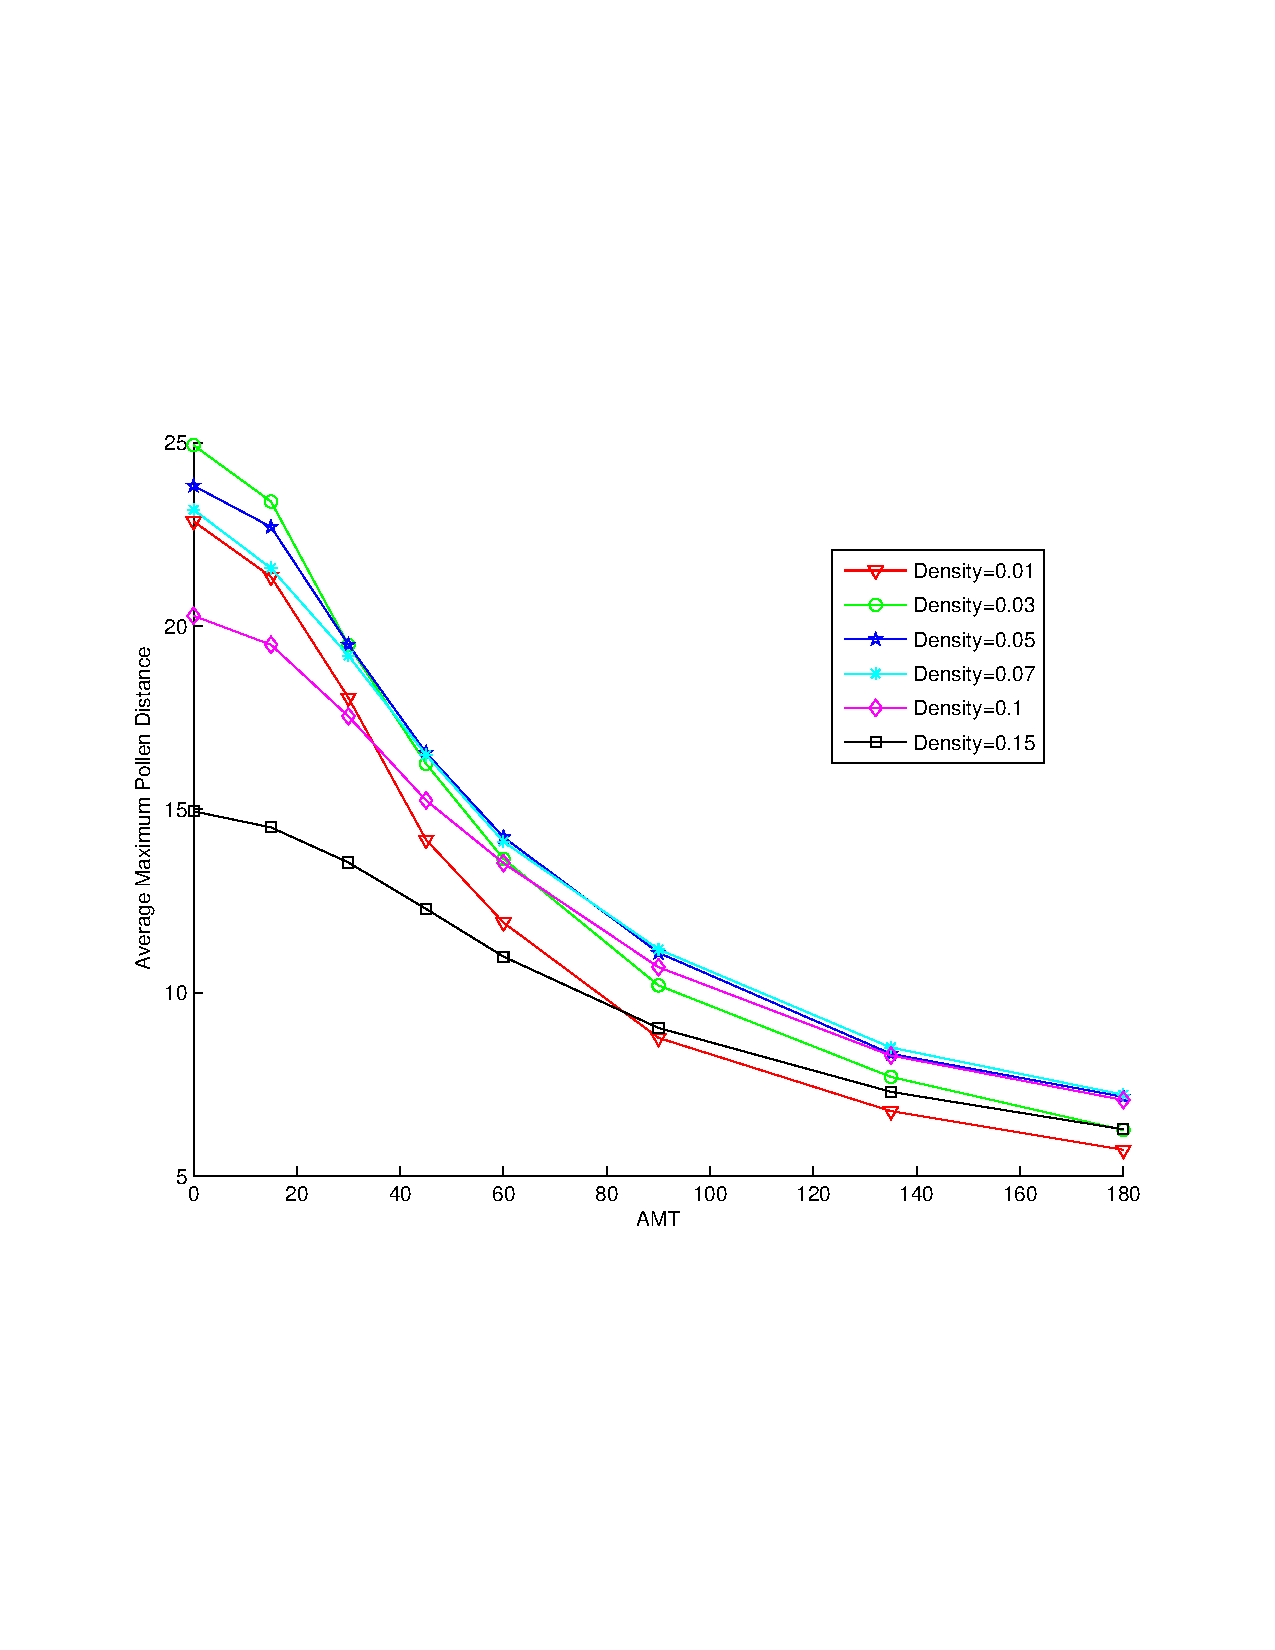
\includegraphics[width=1.0\textwidth]{MaxPollenVsAMT.pdf}
  \end{center}
  \caption{\small Average Maximum Pollination Distance vs. Turning Angle for
Various Plant Densities}
  \label{AvgMaxDTreesN}
\end{figure}

The average maximum pollination distance is clearly affected by the turning
angle, as can be seen in {\bf Figure} \ref{AvgMaxDTreesN}. However, the effect
of plant density on the average maximum pollination distance is unclear, due to
strange behavior observed for low plant densities. The average maximum
pollination distance for both plant densities 0.01 and 0.03, unexpectantly, have
varying behavior across the different turning angles. However, as a general
trend, excluding the 0.01 and 0.03 plant densities, the average maximum
pollination distance decreases as the density increases. This behavior is what
would be expected, since plants are closer together for high densities.

The average maximum pollination distance decreases as AMT increases from
$0^{\circ}$ to $180^{\circ}$ across all densities. This is due to animals
covering a shorter distance for higher turning angles, and therefore the plants
that are visited will be closer together on average. Additionally, we see that
the resultant average maximum pollination distance for a purely random diffusion
process is marketably lower than those for correlated random walks resulting in
straighter animal paths. Thus, wind dispersal will result in an average maximum
pollination distance that is less than the average maximum pollination distance
for a correlated random walk. Thus, one might expect that wind dispersal of
pollen results in a smaller areal extent of gene flow as compared to animal
mediated gene flow.

\subsubsection*{\emph{Average Weighted Diversity of Fathers}}
\begin{figure}
  \begin{center}
  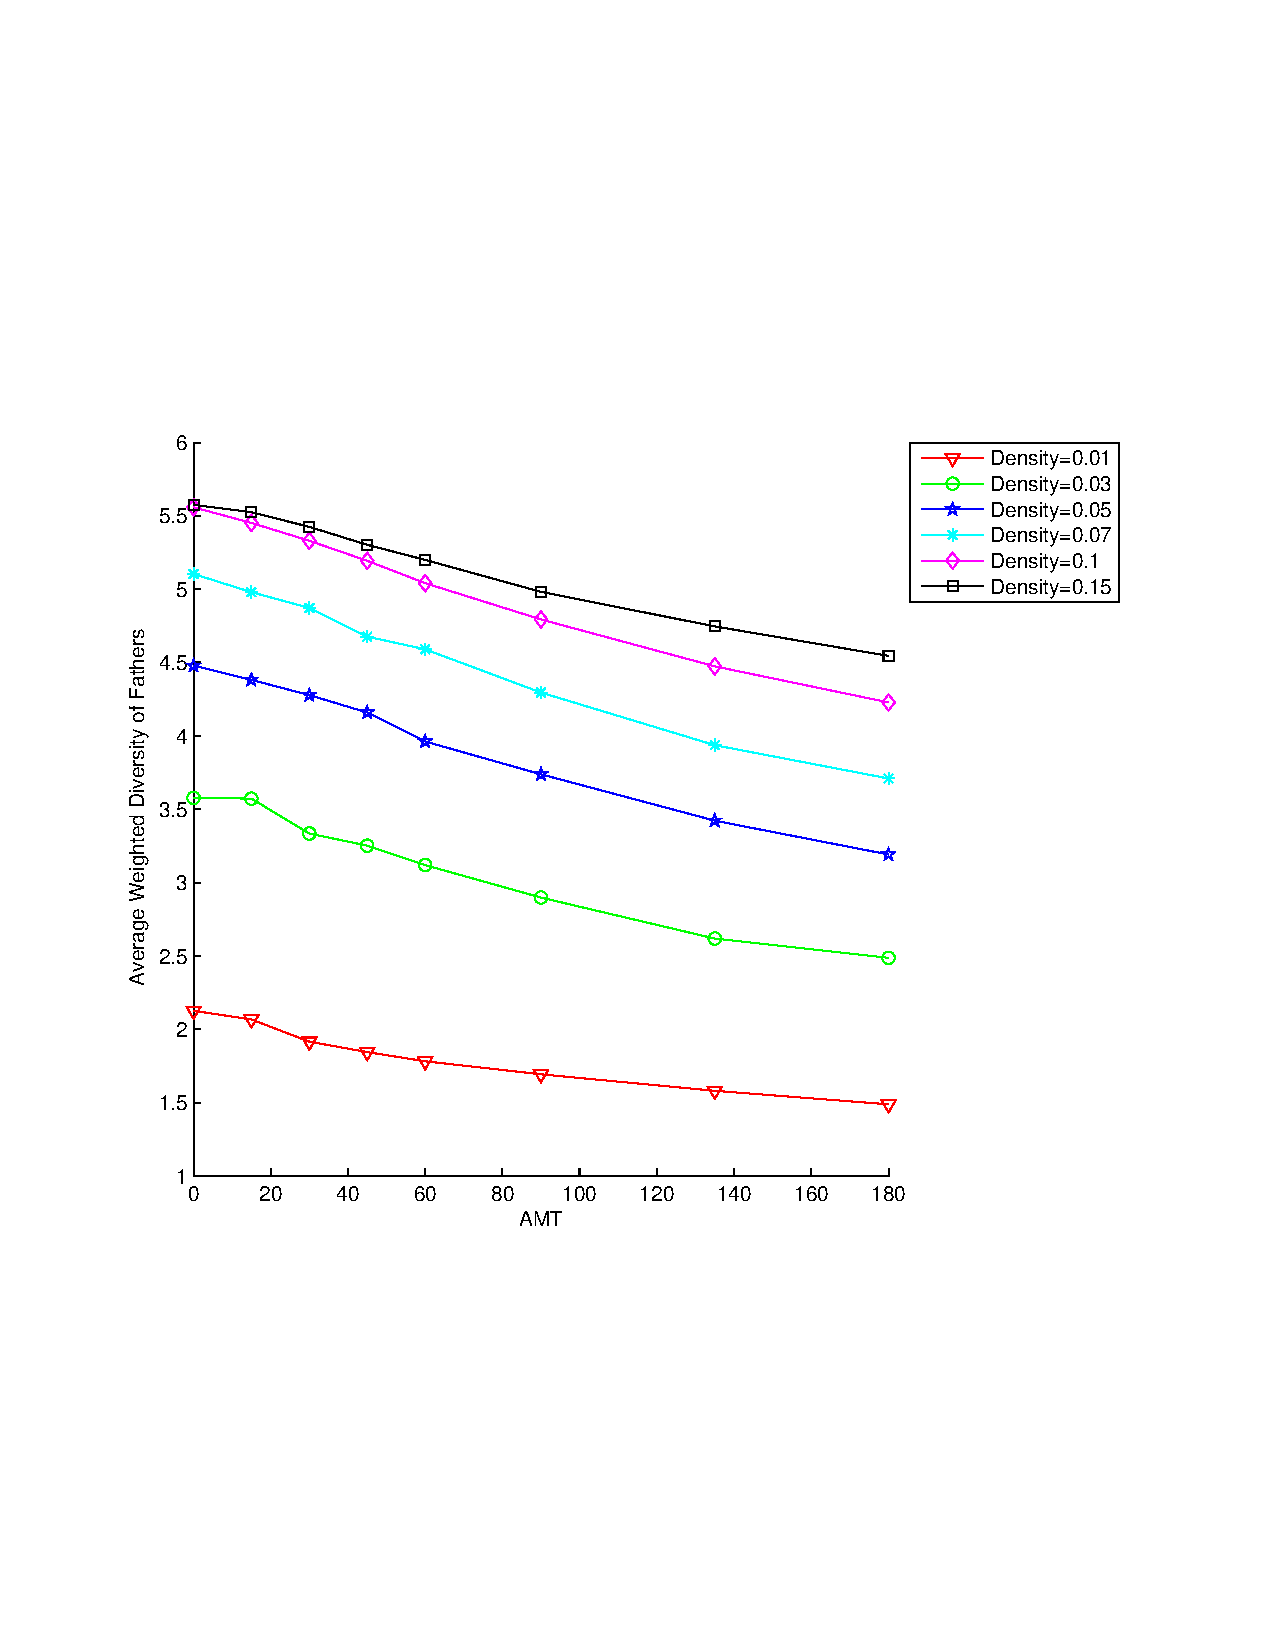
\includegraphics[width=1.0\textwidth]{WDFvsAMT.pdf}
  \end{center}
  \caption{\small Average Weighted Diversity of Fathers vs. Turning Angle for
Various Plant Densities}
  \label{EFathers}
\end{figure}
In general as the turning angle increases the average weighted diversity of
fathers decreases. For a plant density of 0.01 and AMT = $180^\circ$ the average
weighted diversity of fathers is approximately three-quarters of the average
weighted diversity of fathers for the same plant density and AMT = $0^\circ$. This
is likely due to the animal returning to the same plants multiple times for the
larger values of AMT.

The averages weighted diversity of fathers tends to increase, across all values
of turning angle, as density increases. This is due to the availability of more
plants in a shorter distance. Thus, the average weighted diversity of fathers for
wind dispersal will be less than that for animals that travels straighter paths.

\section{{\bf Discussion}}
The majority of models studying pollination have assumed a purely random
diffusion process. However, if the magnitude of an animal's turning angle is
smaller than AMT = $180^\circ$, the results show that significant bias can be
introduced into the analysis of pollination. From the agent based correlated
random walk model presented we can see that significant issues are introduced
when treating animal dispersal as a purely random process when the animals
pollinating may move along straighter paths.

As can be seen in the results section the magnitude of turning angle had varying
degrees of effects over different plant densities and therefore pollination
patterns predicted by a model assuming a purely random walk could be vastly
different from a model assuming a correlated random walk.. For high plant
densities, the effects of correlated random walk was less pronounce than that of
low plant densities, except for the \emph{average weighted diversity of
fathers}. In the case of \emph{average weighted diversity of fathers} the affect
of turning angle magnitudes were more pronounced for high densities. Therefore,
although diffusion models for densely populated plant species may not vary
greatly from models that assume a correlated random walk for \emph{average
pollination distance} or \emph{average maximum pollination distance} they will
vary significantly for \emph{average weighted diversity of fathers}. This has
the affect of under estimating the diversity of pollination for high plant
densities and animal dispersal as compared to similar plant densities and wind
dispersal.

The variation between correlated random walk and that of a purely random walk is
significant at low plant densities for the statistics such as \emph{average
maximum distance}, \emph{average pollination distance}, and \emph{average
maximum pollination distance} and so for the case of low plant densities the
assumption of a purely random walk may lend to bias in the analysis of
pollination. Most studies to date have been conducted on small herbaceous plant
species whose densities tend to be high. Even though most of the animals
statistics presented were not greatly affected by turning angle for high plant
densities the average weighted diversity of fathers had was still greatly
affected by the turning angle at these densities, and therefore an assumption of
a purely random walk would be an inappropriate assumption and at any of the
densities examined in this study. Therefore a correlated random walk may be a
better approximation to animal movement.

\subsection*{Acknowledgment}


%% use the tnoteref command within \title for footnotes;
%% use the tnotetext command for the associated footnote;
%% use the fnref command within \author or \address for footnotes;
%% use the fntext command for the associated footnote;
%% use the corref command within \author for corresponding author footnotes;
%% use the cortext command for the associated footnote;
%% use the ead command for the email address,
%% and the form \ead[url] for the home page:
%%
%% \title{Title\tnoteref{label1}}
%% \tnotetext[label1]{}
%% \author{Name\corref{cor1}\fnref{label2}}
%% \ead{email address}
%% \ead[url]{home page}
%% \fntext[label2]{}
%% \cortext[cor1]{}
%% \address{Address\fnref{label3}}
%% \fntext[label3]{}

\title{}

%% use optional labels to link authors explicitly to addresses:
%% \author[label1,label2]{<author name>}
%% \address[label1]{<address>}
%% \address[label2]{<address>}

\author{}

\address{}

\begin{abstract}
%% Text of abstract

\end{abstract}

\begin{keyword}
%% keywords here, in the form: keyword \sep keyword

%% MSC codes here, in the form: \MSC code \sep code
%% or \MSC[2008] code \sep code (2000 is the default)

\end{keyword}

\end{frontmatter}

%%
%% Start line numbering here if you want
%%
% \linenumbers

%% main text
\section{}
\label{}

%% The Appendices part is started with the command \appendix;
%% appendix sections are then done as normal sections
%% \appendix

%% \section{}
%% \label{}

%% References
%%
%% Following citation commands can be used in the body text:
%% Usage of \cite is as follows:
%%   \cite{key}          ==>>  [#]
%%   \cite[chap. 2]{key} ==>>  [#, chap. 2]
%%   \citet{key}         ==>>  Author [#]

%% References with bibTeX database:

\bibliographystyle{model1a-num-names}
\bibliography{<your-bib-database>}

%% Authors are advised to submit their bibtex database files. They are
%% requested to list a bibtex style file in the manuscript if they do
%% not want to use model1a-num-names.bst.

%% References without bibTeX database:

% \begin{thebibliography}{00}

%% \bibitem must have the following form:
%%   \bibitem{key}...
%%

% \bibitem{}

% \end{thebibliography}


\end{document}

%%
%% End of file `elsarticle-template-1a-num.tex'.
